% !TeX root = ../Skript_HTML.tex
\cohead{\Large\textbf{Links}}
\section{Verlinkungen}
Die Vernetzung von Inhalten über so genannte Links ist ein wesentliches Merkmal des WWW. Aber auch eine normale Homepage besteht in der Regel bereits aus mehreren Seiten, die mit einander verlinkt sind. Man kann aber auch auf die Seiten anderer Anbieter eine Verlinkung setzen.
\begin{minipage}[t]{\textwidth}
    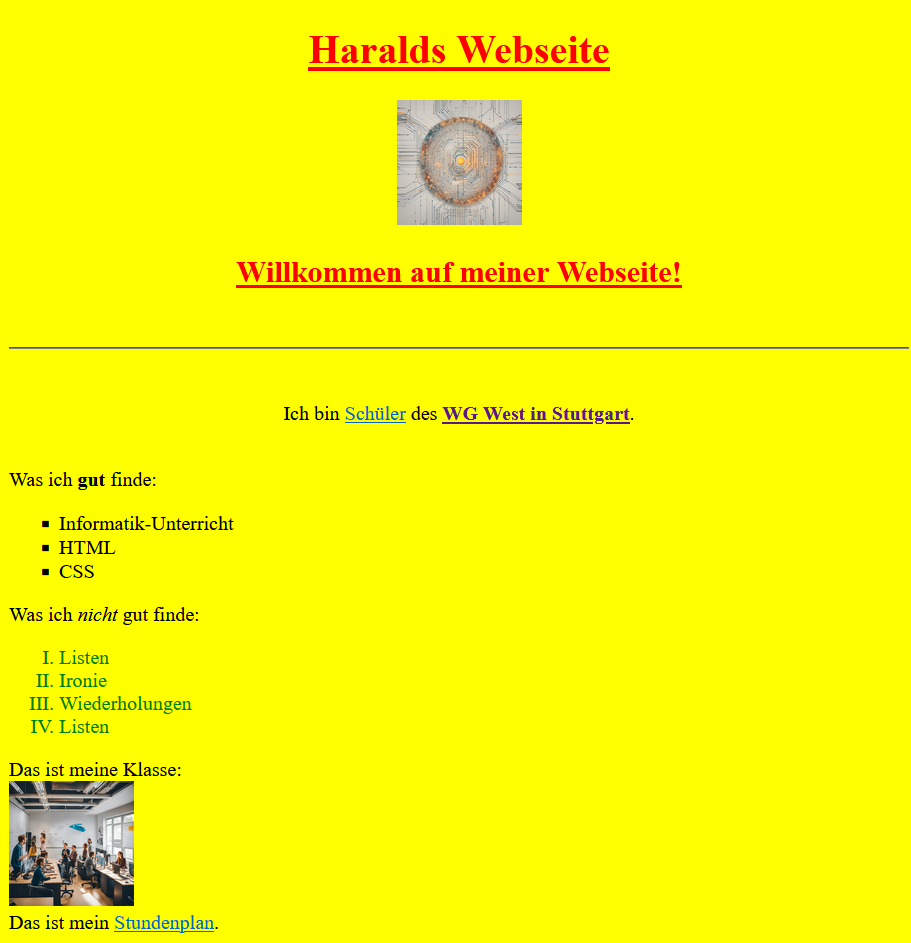
\includegraphics[width=\linewidth]{\pics/Links.png}
\end{minipage}
\begin{Exercise}[title=, label=Links]
    \begin{enumerate}
        \item Erstelle eine Datei \textit{stundenplan.html} im gleichen Ordner wie \textit{schueler.html} mit folgendem Inhalt:
        \begin{lstlisting}
            <!DOCTYPE html>
            <html lang="de">
            <head>
            <link href="style.css" rel="stylesheet" type="text/css">
            <title>Unterricht</title>
            <meta charset="utf-8">
            </head>
            <body>
            So sieht mein Stundenplan aus:
            </body>
            </html>
        \end{lstlisting}
        \item Ergänze deine Webseite wie im Bild zu sehen (du kannst ein beliebiges Bild einbinden. Das Beispielbild wurde mittels \href{https://www.canva.com/}{canva.com} KI-erzeugt). Hinweis: Die beiden Bilder wurden verkleinert, damit das Beispielbild nicht zu groß wird.
        Für das zweite Bild kannst du wieder ein beliebiges Bild aus dem Internet verwenden. Stelle eine Höhe von 400 Pixeln ein.
        \item Erstelle einen Link von WG West in Stuttgart auf die Homepage des WG Wests (\text{https://www.wg-west.de/}).
        \item Erstelle einen Link von Stundenplan auf \textit{stundenplan.html}.
        \item Je nach Größe der eingefügten Bilder ist die Webseite inzwischen so groß, dass nun Scrollen nach unten notwendig ist. Um direkt auf das Bild der Klasse (und weitere Informationen) zu kommen, soll eine Verknüpfung von Schüler direkt auf das Bild führen. Informiere dich über diese Art der Verknüpfung innerhalb einer Datei auf eine ID.
        \item Validiere dann deine Datei \textit{schueler.html}.
    \end{enumerate}
\end{Exercise}